\documentclass[12pt]{article}

\usepackage[spanish, es-tabla, es-nodecimaldot]{babel}
\usepackage[utf8x]{inputenc}
\usepackage{amsmath}

\usepackage{hyperref}
\usepackage{url}
\usepackage{textcomp}
\usepackage{gensymb}
\usepackage[dvipsnames]{xcolor}

\usepackage{parskip}
\usepackage{fancyhdr}
\usepackage{multicol}
\usepackage{vmargin}
\usepackage{setspace}
\usepackage{geometry}

\usepackage{float}
\usepackage{array}
\usepackage{graphicx}
\graphicspath{{images/}}
\usepackage{wrapfig}
\usepackage{caption}
\usepackage{subcaption}

\setmarginsrb{2 cm}{1 cm}{2 cm}{1.5 cm}{0.5 cm}{1 cm}{1 cm}{1 cm} %{izq}{up}{der}{down}{Encabezado}
\title{Eficiencia de Maquinas Térmicas.}
\author{Martín Alejandro Paredes Sosa}		

\makeatletter
\let\thetitle\@title
\let\theauthor\@author
\let\thedate\@date										
\makeatother

\pagestyle{fancy}
\fancyhf{}
%\rhead{Lic.. Física}
%\lhead{Informe 5: \thetitle}
\cfoot{\thepage}

\begin{document}
%====================================================================
\begin{center}
{ \large \bfseries \thetitle}
\end{center}
	\begin{minipage}{\textwidth}
		\begin{center} 
			\theauthor 
			\end{center}
	\end{minipage}
%===================================================================================================
\begin{abstract}
En esta experiencia se utilizó un aparato de eficiencia térmica para transformar energía en forma de calor en eléctrica y viceversa. La máquina opero entre dos temperaturas fijas, de las cuales se midió el voltaje y la corriente asociadas a cada foco para poder obtener la potencia del foco caliente y del foco frío para así poder calcular su eficiencia.
\end{abstract}
\vspace{-1cm}
%===================================================================================================
\section{Introducción}
Esta practica consistió en identificar la eficiencia de una máquina térmica.La eficiencia de una máquina térmica se define como:

\begin{equation}
\eta = \frac{W}{Q_h}
\end{equation}

donde
\begin{itemize}
 \item W es el trabajo hecho por el sistema.
\item $Q_h$ es la energía en forma de calor transferido del baño caliente al sistema.
\end{itemize}

En el caso de una máquina de Carnot la eficiencia tiene la siguiente forma:

\begin{equation}
\eta_c = \frac{T_h - T_c}{T_h}
\end{equation}

donde 
\begin{itemize}
\item $T_h$ es la temperatura del baño térmico caliente
\item $T_c$ es la temperatura del baño térmico frío
\end{itemize}

La eficiencia de la máquina de Carnot es la eficiencia máxima que puede tener una máquina térmica para así no violar la segunda ley de la termodinámica.

\hspace{0.75cm} El objetivo de esta experiencia es calcular la eficiencia del aparato de Peltier el cual transforma energía en forma de calor en energía eléctrica.

Este aparato opera entre dos temperaturas fijas, las temperaturas $T_h$ y $T_c$, éstas son medidias con termistores que están puestos en los bloques de aluminio.
Este aparato mide la razón a la cual la energía es transferida, es decir, mide la potencia, de tal forma que si la energía transferida es $Q_h$ por unidad de tiempo, la potencia será:

\begin{equation}
P_h = \frac{dQ_h}{dt}
\end{equation}

Si expresamos primera ley en términos de potencia, tenemos:

\begin{equation}
P_h = P_W + P_c
\end{equation}

Así la eficiencia de ésta máquina es 
 
\begin{equation}
\eta = P_w + P_h
\end{equation}

donde $P_h$ está determi
Si expresamos primera ley en términos de potencia, tenemos:

\begin{equation}
P_h = P_W + P_c
\end{equation}

Así la eficiencia de ésta máquina es 
 
\begin{equation}
\eta = \frac{P_w}{P_h}
\end{equation}

donde $P_h$ está determinada por el voltaje y la corriente de entrada que calienta el bloque de alumnio, o sea

\begin{equation}
P_h = V_h I_h
\end{equation}

$P_W$ será la energía eléctrica producida por el aparato Peltier el cual a su vez conduce una corriente a tráves de una resistencia $R_0$ que tiene un voltaje $V_0$, así

\begin{equation}
P_W = \frac{V_0^2}{R_0}
\end{equation}
\vspace{-0.5cm}
%===================================================================================================
\section{Desarrollo Experimental}
\vspace{-0.5cm}
El montaje experimental se ilustra en la siguiente figura:

\begin{figure}[H]
\begin{center}
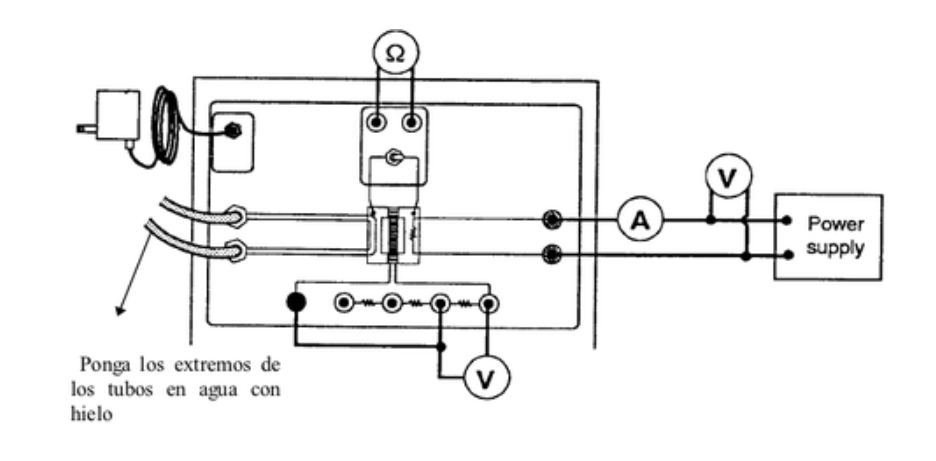
\includegraphics[width=0.8\textwidth]{Arreglo.png}  
\caption{Diagrama aparato Peltier}
\label{one}
\end{center}
\end{figure}

Como se puede observar en la figura, del lado izquierd se encuentran dos mangueras que permiten recircular el agua fría y por el lado derecho está conectada una fuente que suministra la energía eléctrica que mantendrá la temperatura del baño caliente.

En los sitios marcados con circulos se midieron la resistencia, el voltaje y la corriente.

El procedimiento se resume en la siguiente lista:
Partiendo del arreglo mostrado en la figura.
\begin{itemize}
\item Se conectó las dos mangueras al baño frío.
\item Se conectó la fuente de corriente con un voltaje fijo de
aproximadamente 2 volts.
\item Se midió el voltaje $V_0$ lo cual y se fijo la resistencia $R_0$ en 2 ohms.
\item Se midió la corriente $I_h$ en el amperímetro, el cual fue conectado en serie con la fuente de corriente del lado derecho.
\item Se repitieron las mismas condiciones anteriores pero con valores de voltaje $V_h$ de 3,4,5 y 6 volts.
\end{itemize}
%===================================================================================================

\section{Resultados}
Las mediciones hechas se presentan en la siguiente tabla:

	\begin{table}[H]
		\centering
		\begin{tabular}{|cccccccccc|}
			\hline
			$T_c$ (K)&$T_h$ (K)&$T_c$ ($^0C$)&$T_h$ ($^0C$) & $V_h$ (V) & $I_h$ (A) &$R_0 (\Omega)$ & $V_0 (V)$ & $P_h$ (W) & $P_W$ \\ \hline
			275&  279.5& 3& 6.5&  2 & 0.362& 2 &0.084 &0.724 & 3.52 mW\\ \hline
			275.9 &281.2 &2.9 &8.2 & 3& 0.546& 2& 0.091& 1.638& 4.14 mW\\ \hline
			276.3 &285.3 &3.3 &12.3 &4 & 0.728 &2 &0.132 & 2.912& 8.712 mW\\ \hline
			276.7 &289.7 &3.7 &16.7 &5 & 0.914 &2 &0.195 &4.57 & 0.0190 W \\ \hline
			277.4 &295.5 &4.4 &22.5 &6 & 1.102 &2 &0.275 & 6.612 & 0.037 W\\ \hline
		\end{tabular}
		\caption{Mediciones}
		\label{tab:traIso}
	\end{table}

En la siguiente tabla, se muestra el valor de la eficiencia dependiendo $V_h$:
\begin{table}[H]
\centering
\begin{tabular}{|ccc|}
\hline
$V_h$ (V)& $\eta$ & $\eta_c$ \\ \hline
2& 4.861 $ \times 10 ^{-3}$ & 0.02 \\ \hline
3&2.527 $ \times 10 ^{-3}$ & 0.018\\ \hline
4& 2.991 $ \times 10 ^{-3}$& 0.031\\ \hline
5& 4.157 $ \times 10 ^{-3}$& 0.044 \\ \hline
6& 5.595 $ \times 10 ^{-3}$& 0.061 \\ \hline
\end{tabular}
\caption{Valores obtenidos de la eficiencia}
\label{tab:taIso}
\end{table}

La siguiente gráfica presenta la $\frac{1}{T_h}$ vs $\eta$:

	\begin{figure}[H]
		\centering
		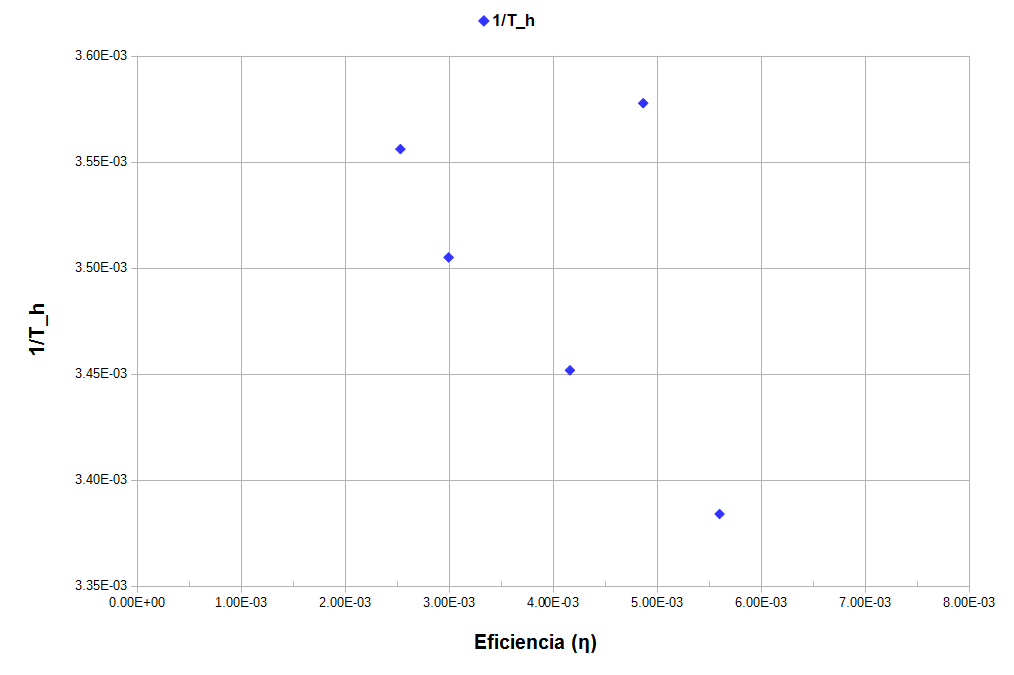
\includegraphics[width=\textwidth , height = 10cm]{1-TvsNMal.png}  
		\caption{$\frac{1}{T_h}$ vs $\eta$}
		\label{nMal}
	\end{figure}

La siguiente gráfica presenta la $\frac{1}{T_h}$ vs $\eta_c$:

	\begin{figure}[H]
		\centering
		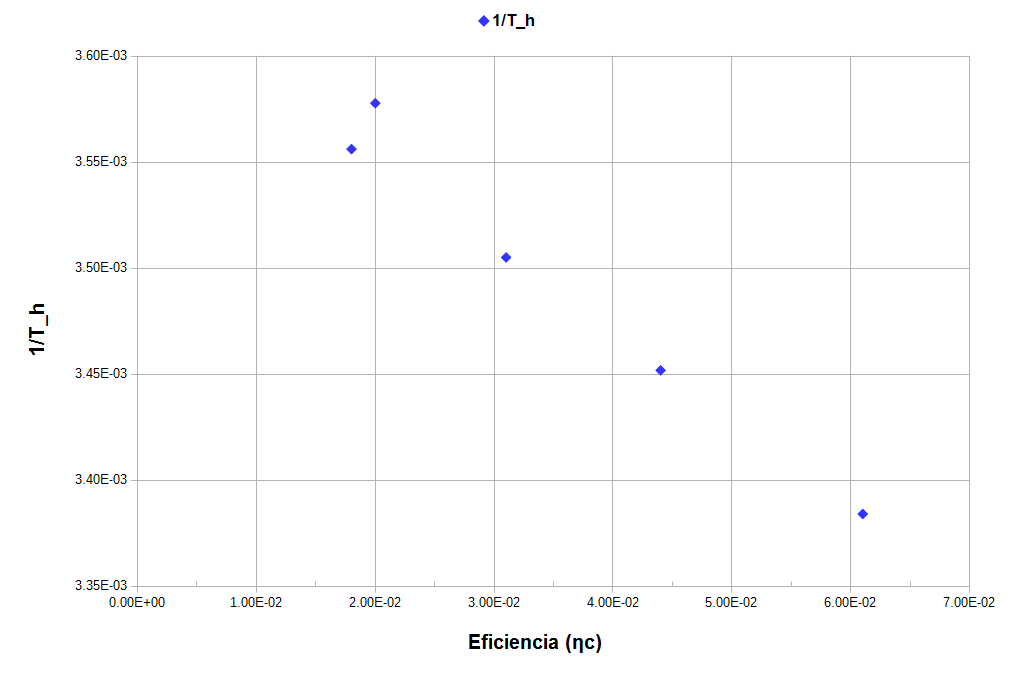
\includegraphics[width=\textwidth , height = 10cm]{1-TvsNcMal.png}  
		\caption{$\frac{1}{T_h}$ vs $\eta_c$}
		\label{ncMal}
	\end{figure}


Se puede apreciar que hay un valor que no pertenece. Como el primer dato no concuerda con los demás, se procedió a omitir el dato en los resultados. Esto se puede deber a un error durante el experimento, ya sea no se tomo el tiempo suficiente, o un error al medir. Las siguintes graficas muestran los resultados que se obtienen omitiendo el primer dato:

La siguiente gráfica presenta la $\frac{1}{T_h}$ vs $\eta$:

	\begin{figure}[H]
		\centering
		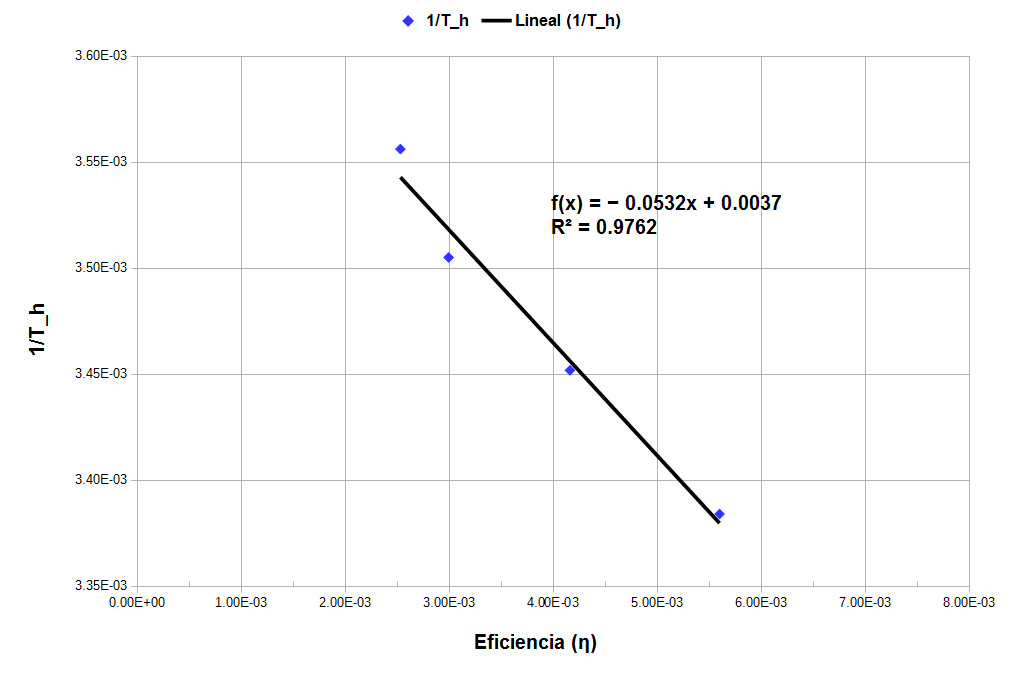
\includegraphics[width=0.75\textwidth , height = 7cm]{1-TvsN.png}  
		\caption{$\frac{1}{T_h}$ vs $\eta$}
		\label{n}
	\end{figure}

La siguiente gráfica presenta la $\frac{1}{T_h}$ vs $\eta_c$:

	\begin{figure}[H]
		\centering
		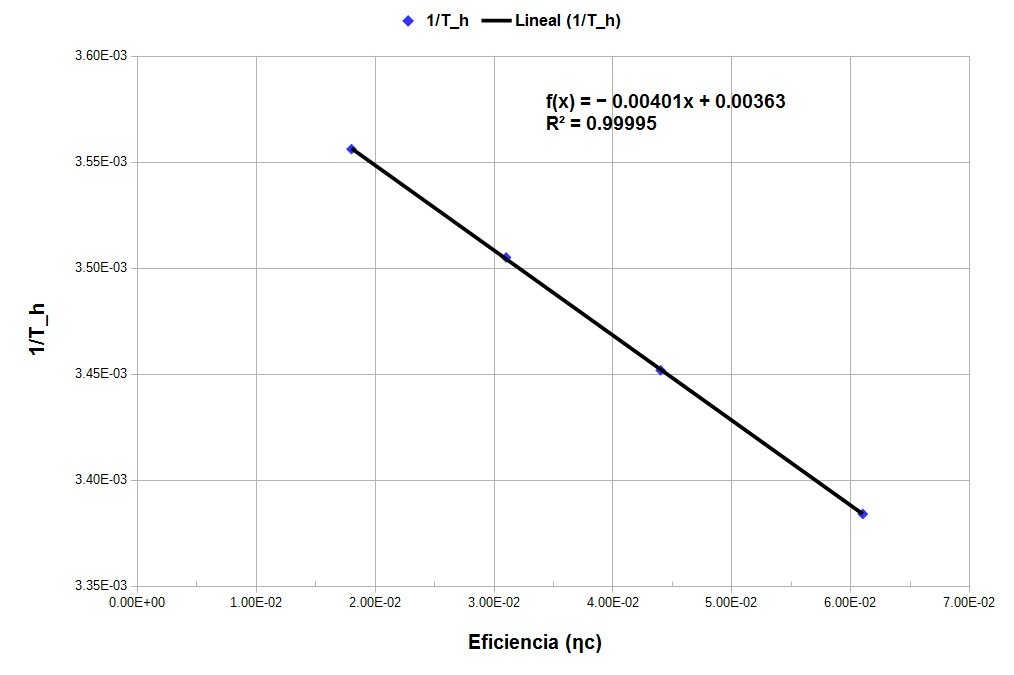
\includegraphics[width=0.75\textwidth , height = 7cm]{1-TvsNc.png}  
		\caption{$\frac{1}{T_h}$ vs $\eta_c$}
		\label{nc}
	\end{figure}
%===================================================================================================	
\section{Discusiones}
En este trabajo se observo como se relaciona la temperatura de con la eficiencia. Se observo que la eficiencia siempre fue menor a la de Carnot, como se encuentra en los libros, no tenemos una maquina que rompe la segunda Ley. También se vio que al aumentar la temperatura del foco caliente, la eficiencia de la maquina disminuye.
%===================================================================================================
\section{Conclusiones}
La eficiencia disminuye linealmente al aumentar el voltaje fijo ($V_h$), de las gráficas se puede notar que la eficiencia real siempre es menor que la eficiencia de Carnot, esto debido a que la eficiencia de Carnot es la máxima eficiencia que se puede obtener. 

Realizando un ajuste lineal obtuvimos una recta mejor definida en el caso de la eficiencia de Carnot.
Estos dos resultados se deben al primer teorema de Carnot que dice "No puede existir una máquina térmica que funcionando entre dos fuentes térmicas dadas tenga mayor rendimiento que una de Carnot que funcione entre esas mismas fuentes térmicas." 
Calculando el promedio de las eficiencias se obtuvo que la eficiencia de la máquina de Peltier es 10$\%$ la eficiencia de la máquina de Carnot.

Las fuentes de error fueron diversas, desde no esperar a que el sistema se estabilizara hasta cálculos érroneos de las temperaturas.
%================================================================================================


\begin{thebibliography}{6}


\bibitem{acu}
Acuña, H. (2015). \textit{Manual de Guías de Experiencias en el Laboratorio de Termodinámica Clásica}.

\bibitem{W}
Zemansky, M., Dittman, R.(1990) \textit{Calor y Termodinámica}


\end{thebibliography}
%================================================================================================


\end{document}
